To obtain a measure of the Fierz term, the beta decay spectrum must be precisely described.
The description of the beta decay spectrum is writen as a series of corrections on top of the main phase space factor.  

The corrections depend on several parameters of the decay. 
Some of them are just numbers, such as the atomic number of the daughter or mother nucleus or the mass number of the system.
However, there are two important paramters that are inexact.
They are measured experimentally.

One is the q-value of the decay, which is defined in equation \ref{eq:qval}.

\begin{equation}
	Q = m_{p} - (m_{d} + E_{\gamma})
	\label{eq:qval}
\end{equation} 
where $Q$ is the q-value, $m_{p}$ is the mass of the parent nucleus, $m_{d}$ is the mass of the daughter nucleus, and $E_{\gamma}$ is the energy of any gamma rays in the decay.
For this measurement, the atomic mass of $^{20}$Ne and $^{20}$F were used \cite{Pfe12}.
The mass of the electrons subtracts out atomic masses, since in neutral fluorine there are nine electrons, and one electron is gained from the beta decay.
This then equals the ten electrons in the atomic mass of neon.
The only correction missing is the small, eV scale electron binding energy of the last electron.

The other parameter is the charge radius of the daughter nucleus.
There are several ways to calculate the charge radius.
In this work, the charge radius was taken from the measured RMS charge radius and converted.
It was assumed that the $^{20}$Ne nucleus was a sphere. 
From this, the radius was calculated using equation \ref{eq:sphereeq}

\begin{equation}
	r = \sqrt{\frac{5}{3}}r_{rms}	
	\label{eq:sphereeq}
\end{equation}

where $r_{rms}$ is the root mean square radius, and $r$ the charge radius.

With the two parameters, the q-value and the phase space, the shape of all beta decay spectra can be described.

\section{Phase Space Beta Decay}
The main part of the beta decay spectrum is the phase space factor.
It is shown in equation \ref{eq:phase_space}

\begin{equation}
	\frac{dN}{dE} = C * p_{\beta}W(Q - W)^{2}
	\label{eq:phase_space}
\end{equation}

were $C$ is a constant which includes the matrix element squared, $p_{\beta}$ is the beta momentum, $W$ the total electron energy, and $Q$ the q-value of the beta decay.
This is derived from the density of states of the particle.
This comes in from Fermi's Golden Rule, which is shown in equation \ref{eq:fgr}.

\begin{equation}
	\lambda = \frac{2\pi}{\hbar}\|M\|^{2}\rho
	\label{eq:fgr}
\end{equation}

where $\lambda$ is the transition probablity, $M$ the matrix element, and $\rho$ the density of the states.
The main effect on the spectrum shape originates from the density of states.
The number of states for both the electron and the neutrino is show in equation \ref{eq:densityofstates}

\begin{equation}
	N = \frac{1}{(2\pi\hbar)^{6}}\int dr^{3}_{\beta} \int dp^{3}_{\beta}\int dr^{3}_{\nu_{e}} \int dp^{3}_{\nu_{e}} 
	\label{eq:densityofstates}
\end{equation}

where $r$ and $p$ corresponds to the position and momentum of the electron ($\beta$) and the neutrino ($\nu_{e}$).
Doing the integral over both $r$'s give two factors of the volume, which disappear when the next factor is introduced.
Since the neutrinos are unmeasured, the momentum of the neutrinos is integrated over. 
Assuming spherical symmetry, the new integral is shown in equation \ref{eq:dosspherical}

\begin{equation}
	dN = \frac{V^{2}}{4\pi^{4}\hbar^{6}}p_{\beta}^{2}dp_{\beta}p_{\nu_{e}}^{2}dp_{\nu_{e}}
	\label{eq:dosspherical}
\end{equation}

This is simplfied by approximating the neutrino as massless.
The momentum of the neutrino is then equal to the energy of the neutrino.
Then, the total energy $E$ is written as a sum of the neutrino energy (or momemntum) and the beta energy.
Plugging that in gives equation \ref{eq:dosintegral} after integrating over the neutrino degrees of freedom. 

\begin{equation}
	dN = \frac{V^{2}}{4\pi^{4}\hbar^{6}}(E - E_{beta})^{2}p_{\beta}^{2}dp_{\beta}
	\label{eq:dosintegral}
\end{equation}

Then, the only thing left to do to recover equation \ref{eq:phase_space} is to rewrite $dp$ in terms of $dE$. 
The energy $E_{beta}$ has been replaced with $W$, which is the energy of the electron divided by the mass an electron, and $E$ has been replaced by the Q-value.
Since the measurement is not an absolute one, but only concerned with the shape of the spectrum, the normalization factor is arbitrary.

This is the main factor in describing the beta decay energy spectrum.

\subsection{Matrix Elements}
In the above disccusion, the matrix elements of the beta decay was glossed over.

INSERT DISCUSSION HERE
\section{Variables of Correction Formula}

For the rest of the discussion on beta decay corrections, everything is given without units.
All of the energies are divided by the electron mass, i.e. 511 keV.
The other important variables are shown in table \ref{tab:vars}

\begin{table}[!hbt]
	\centering
	\caption{Variables used in the theory corrections}
	\resizebox{\textwidth}{!}{
		\begin{tabular}{r|l|l}
		Variable & Description & Equation or Value \\ \hline		
		$A$ & Mass number & 20 \\ 
		$Z$ & Atomic number of daughter & 10 \\
		$\alpha$ & Fine structure constant & 1/137.0359\\
		$R$ & Root mean square charge radius of daughter & 3.055 fm \cite{Ang13} \\
		$W$ & Total energy of beta electron & $E/m_{e}$ \\
		$p$ & Electron momentum & $\sqrt{W^{2} - 1}$ \\
		$W_{0}$ & Maximum electron energy & $\frac{M_{^{20}F} - M_{^{20}Ne} - E_{gamma ray}}{m_{e}}$ \\
		$\gamma$ & Factor that shows up in EM corrections& $\sqrt{1 - (\alpha Z)^{2}}$ 
		\end{tabular}}
	\label{tab:vars}
\end{table}

To convert the RMS charge radius into the regular charge radius, it is assumed that the nucleus was a sphere. 
This means multiplying the radius given in table \ref{tab:vars} by $\sqrt{\frac{3}{5}}$.
Finally, in order to put it into natural units, the result was divided by the reduced Compton wavelength of the electron.

The two factors that require experimental input were $R$ and $E_{0}$. 
$R$ was given directly in data tables.
For $E_{0}$, the mass of $^{20}$F and $^{20}$Ne were needed.
The energy of the gamma ray photon was also needed.
Each one of these had an uncertainty, which propogates through the various correction functions.
Before the theoretical corrections were fed into a Monte Carlo simulation, the uncertainties were checked.
Theoretical spectra were  built with each value plus or minus it's uncertainty.
Ratios between the spectra were taken and fit with a line.
The results of those ratios are seen in figure \ref{fig:theoryuncer}.

\begin{figure}[!htb]
	\centerline{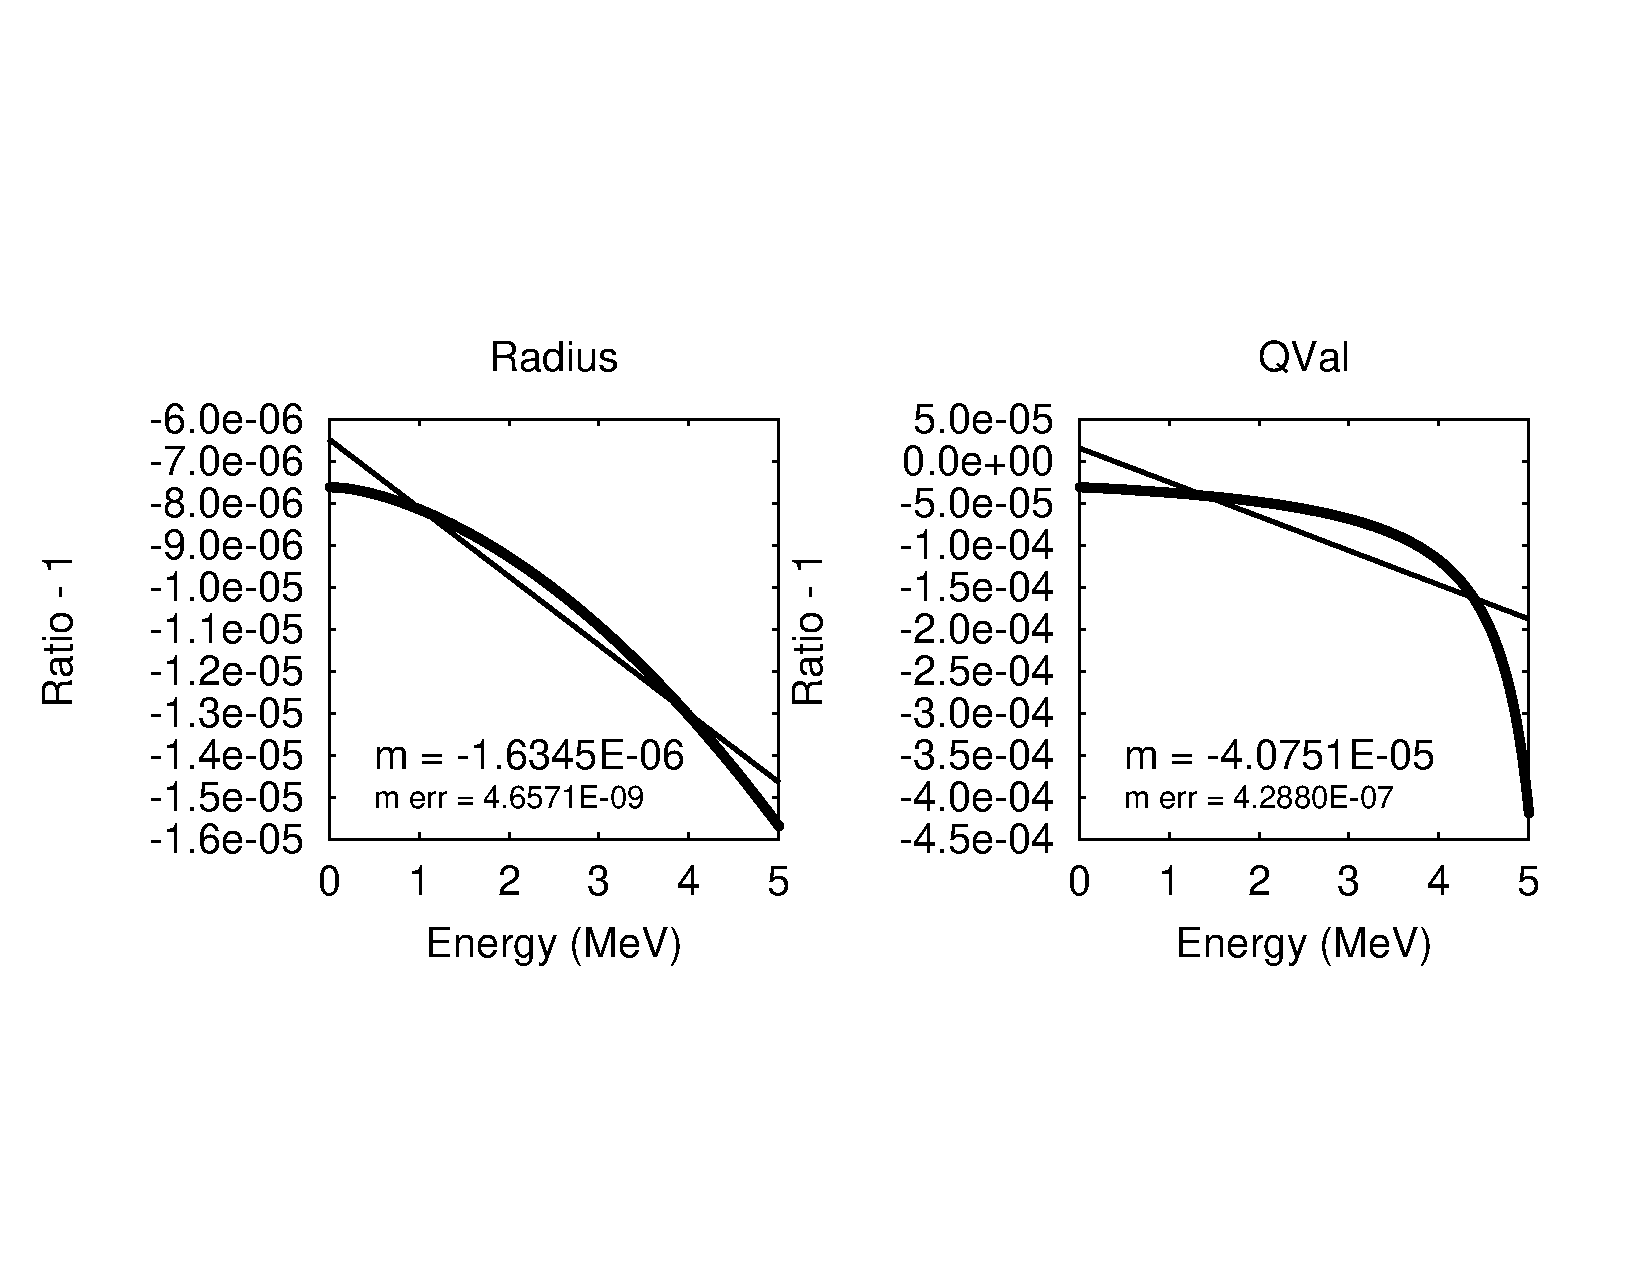
\includegraphics[width=0.78\textwidth]{RatioPlot_2.pdf}}
	\caption{An estimate of the theory uncertainty due to the experimental parameter uncertainty.	
		 Shown are the slopes for each experimental parameter. 
		 They are orders of magnitude smaller than the $10^{-2}$/MeV of the $C_{1}$.}
	\label{fig:theoryuncer}
\end{figure}

Since the slopes of each line are much smaller than the shape factor values, the experimental uncertainties are negligable. 
The various theoretical corrections that are needed are now discussed below.

\section{Fermi Function}

The largest correction. 
This accounts for the interaction of the charge of the outgoing electron and the charge of the nucleus.
It is calculated by taking the Dirac equation wave functions and assuming the nucleus is a point charge of Ze.
The Dirac wave functions are taken down to a nuclear radius R.
This is since the wave functions diverge \cite{Wil89}.

The Fermi function is printed in equation \ref{eq:fermifunc}

\begin{equation}
	F(Z,W) = 2\frac{\gamma + 1}{\Gamma(2\gamma +1)^{2}}(2pR)^{2(\gamma - 1)}e^{\frac{\pi\alpha ZW}{p}}\|\Gamma(\gamma + i\frac{\alpha ZW}{p}\|^{2}
	\label{eq:fermifunc}
\end{equation}

While this is the largest correction, it is the most understood one.
It also only depends on one parameter with experimental uncertainty, $R$. 


\section{Radiative Correction}
The radiative correction was the next largest correction.
For this measurement, the correction is only need to first order, which is on order $\alpha$.
The correction is a QED correction that stems from photons emitted from the beta particle.
This photon can be absorbed by the nucleus of the daughter, which makes it a virtual photon.
The photon can also be a real photon that propogates out off to inifinity.
The real photons are known as inner bremsstrahlung.

There are different descriptions of the radiative correction.  
The first is by Sirlin \cite{Sir67} and is shown in equation \ref{eq:sirlinrad}.

\begin{equation}
	\resizebox{.9\textwidth}{!}
	{
	$R(W,W_{0}) = 1 + \frac{\alpha}{2\pi}[3ln(M) - \frac{3}{4} + 4(\frac{arctanh(\beta)}{\beta} - 1)*(\frac{W_{0} - W}{3W} - \frac{3}{2} + ln(2(W_{0} - W))) + \frac{4}{\beta}L(\frac{2\beta}{1 + \beta}) + \frac{arctanh(\beta)}{\beta}*(2*(1 + \beta^{2}) + \frac{(W_{0} - W)^{2}}{6W^{2}} - 4 arctanh(\beta)]$
	}
	\label{eq:sirlinrad}
\end{equation} 

with $\beta = \frac{p}{W}$, $M$ the proton mass, and $L(\frac{2\beta}{1+\beta})$ referening to the Spence function, as seen in equation \ref{eq:spence} \cite{Wil95}

\begin{equation}
	L(x) = \int_{0}^{x} \frac{ln(1 - t)}{t}dt
	\label{eq:spence}
\end{equation}

The Sirlin formula assumes that the inner bremsstrahlung photons are not detected at all.
This is mostly true if the source of the beta decay is centered outside of a detector.
However, if the source is implanted inside of the detector, such as it is in this experiment, some of the inner bremsstrahlung is absorbed.

If it is all absorbed, a different form of the first order radiative correction is needed.
There are many equivalent forms of this, but the one that was used for this experiment was by Fayans \cite{Fay86}.
The form of this radiative correction is shown in equation \ref{eq:fayansrad}

\begin{equation}	
	\resizebox{.9\textwidth}{!}
	{
	$R(W,W_{0}) = 1 + \frac{\alpha}{\pi}[(\frac{2}{\beta}ln(\frac{2\beta}{1+\beta}) + \frac{7}{8\beta} + \frac{3\beta}{8})ln(\frac{1 + \beta}{1 - \beta}) - 2ln(\frac{4\beta^{2}}{1 - \beta^{2}}) + \frac{4}{\beta}L(\frac{2\beta}{1+\beta}) + \frac{23}{8} + \frac{3}{2}ln(M)]$
	}
	\label{eq:fayansrad}
\end{equation}

With all the functions and variables meaning the same as in equation \ref{eq:sirlinrad}.

Unfortunately, the amount of inner bremssstrahlung absorbed depends on the geometry.
A more careful treatment of the radiative correction was used.

\subsection{Inner Bremmsstrahlung}

To first order, the energy spectrum of the inner bremsstrahlung photons is independent of Z.
This is exactly like the two radiative corrections shown in equations \ref{eq:sirlinrad} and \ref{eq:fayansrad}. 
The spectrum is written out in equation{\ref{eq:KUB} \cite{Kni36}

\begin{equation}
	\Phi(k,W_{e}) = \frac{ \alpha p}{ \pi p_{e} k} ( \frac{W_{e}^{2} + W^{2}}{W_{e}p}log(W + p) - 2 )
	\label{eq:KUB}
\end{equation}

where $\Phi(k,W_{e})$ is the probability density of seeing a photon of energy $k$ from an electron of initial energy $W_{e}$.
This equation was derived one way using outgoing waves from the Dirac equation in polar coordinates.
The first order Born approximations was used.
This means that at low energies, equation \ref{eq:KUB} is inaccurate. 
That can be seen, as the equation diverges as $k$ goes to zero.
If more orders of the approximation are added, this diveregence can be controlled.
These higher orders would correspond to emitting multiple photons.
Each of these orders would have a probablity reduced by a factor of $\alpha$ compared to equation \ref{eq:KUB}.
The higher orders would be less significant, expect for at low energies. 
Since the probablity density diverges, the higher orders could contribute.
This would make the probablity of emitting no photons finite.	 		

However, another possiblity is to add a cutoff. 
As long as the cutoff is high enough to be in the region where the first order Born approximation is valid, but low enough not to cut out gamma rays that are not full absorbed, equation \ref{eq:KUB} is usable.
The cutoff used was 50 keV.
This cutoff was checked using Monte Carlo, and is within the region where the detector and the source geometry absorbs all gamma rays.

To quantify the exact effect of the inner bremsstrahlung, a GEANT4 simulation was used.
Electrons were generated using the phase space and the radiative correction in equation \ref{eq:fayansrad}.
Then, for each electron, equation \ref{eq:KUB} was sampled and a photon generated.
No other physics process was looked at in this simulation.
The ratio consisting of the energy absorbed over the initial energy was the output of the simulation.
That ratio is the effective efficiency of absorbing the inner bremsstrahlung photons.
Multiplying that ratio by equation \ref{eq:fayansrad} gives the effective radiative correction.
Comparing all three radiative corrections can be seen in figure \ref{fig:rad}

\begin{figure}[!htb]
	\centerline{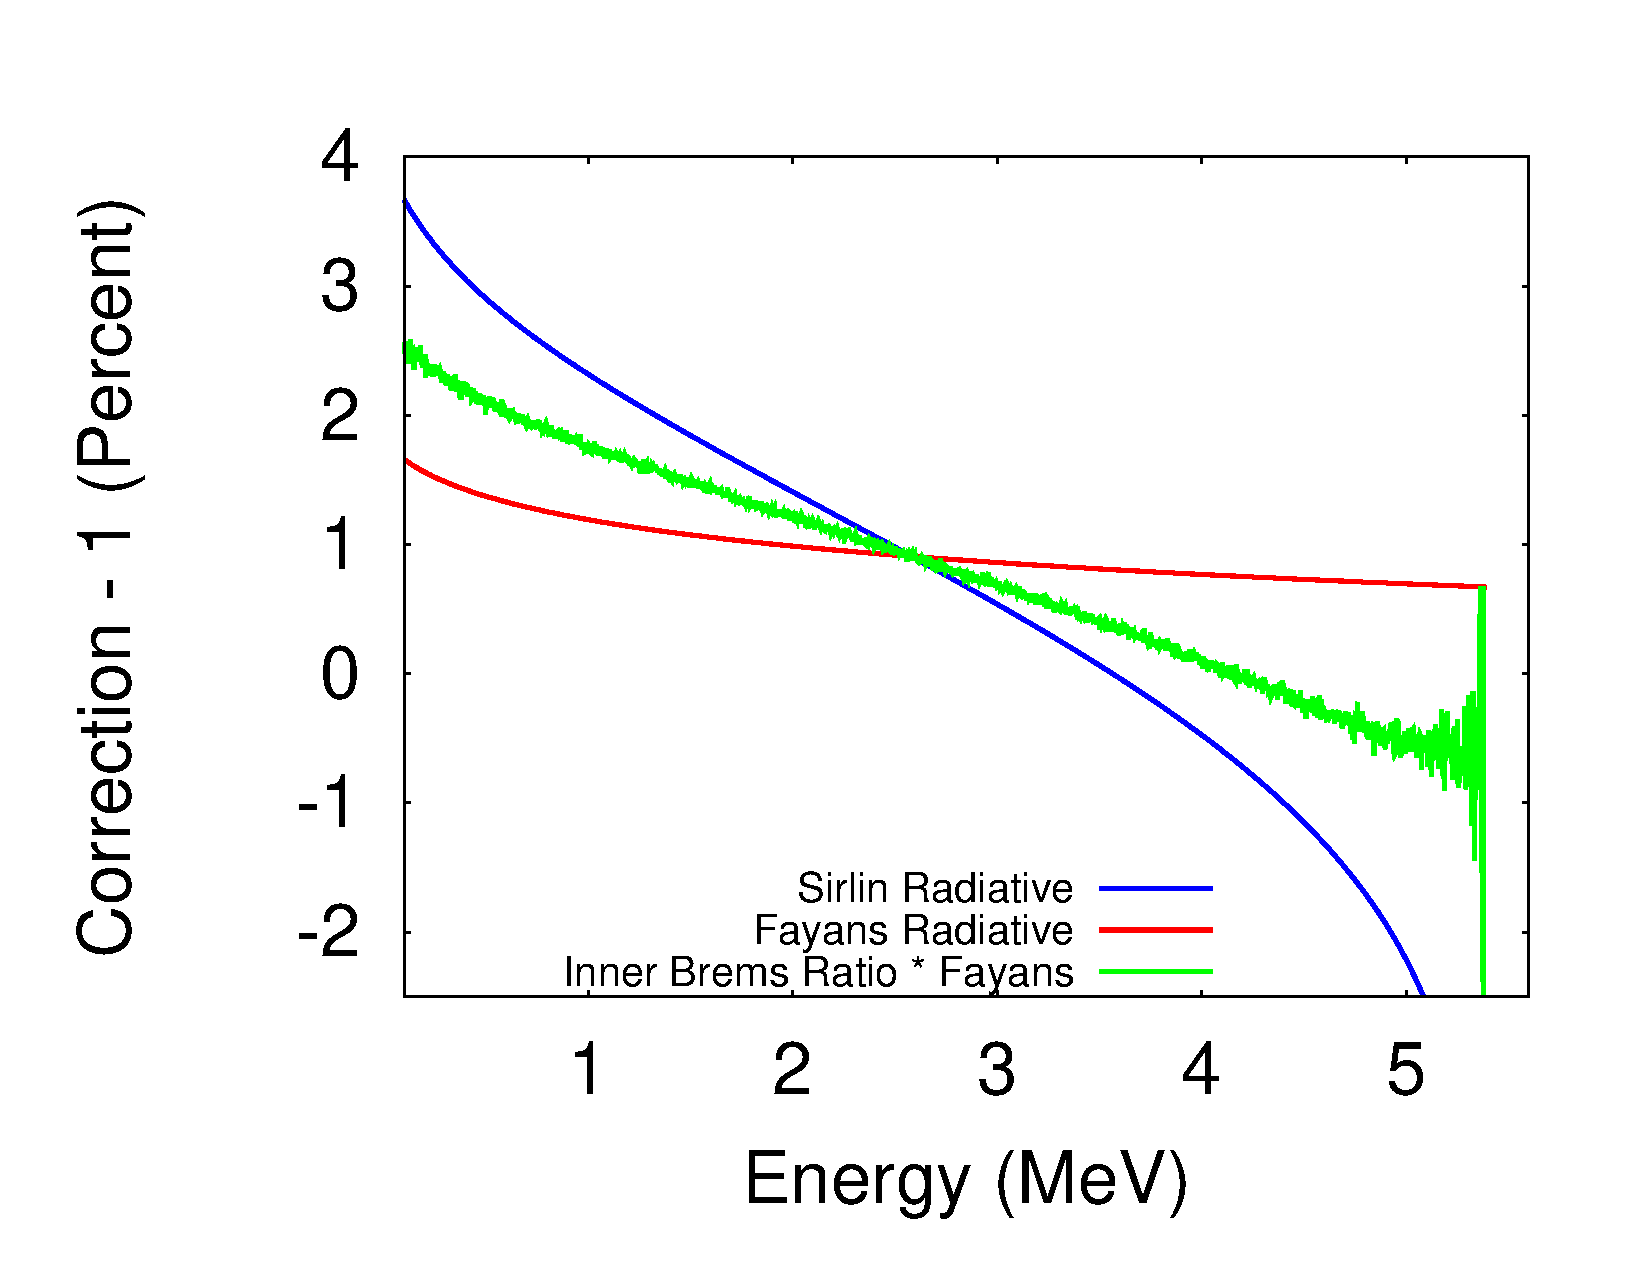
\includegraphics[width=0.78\textwidth]{RadCorrections_20F.pdf}}
	\caption{Comparing three different radiative corrections.
		 The green line depends strongly on the detector geometry}
	\label{fig:rad}
\end{figure}

In order to see the effect of each correction on the slope, all three corrections offset in order to start from the same starting point.
This is seen in figure \ref{fig:radmatch}.
The effect of the inner bremsstrahlung is to put the radiative correction halfway between the Sirlin and the Fayans formulas.

\begin{figure}[!htb]
	\centerline{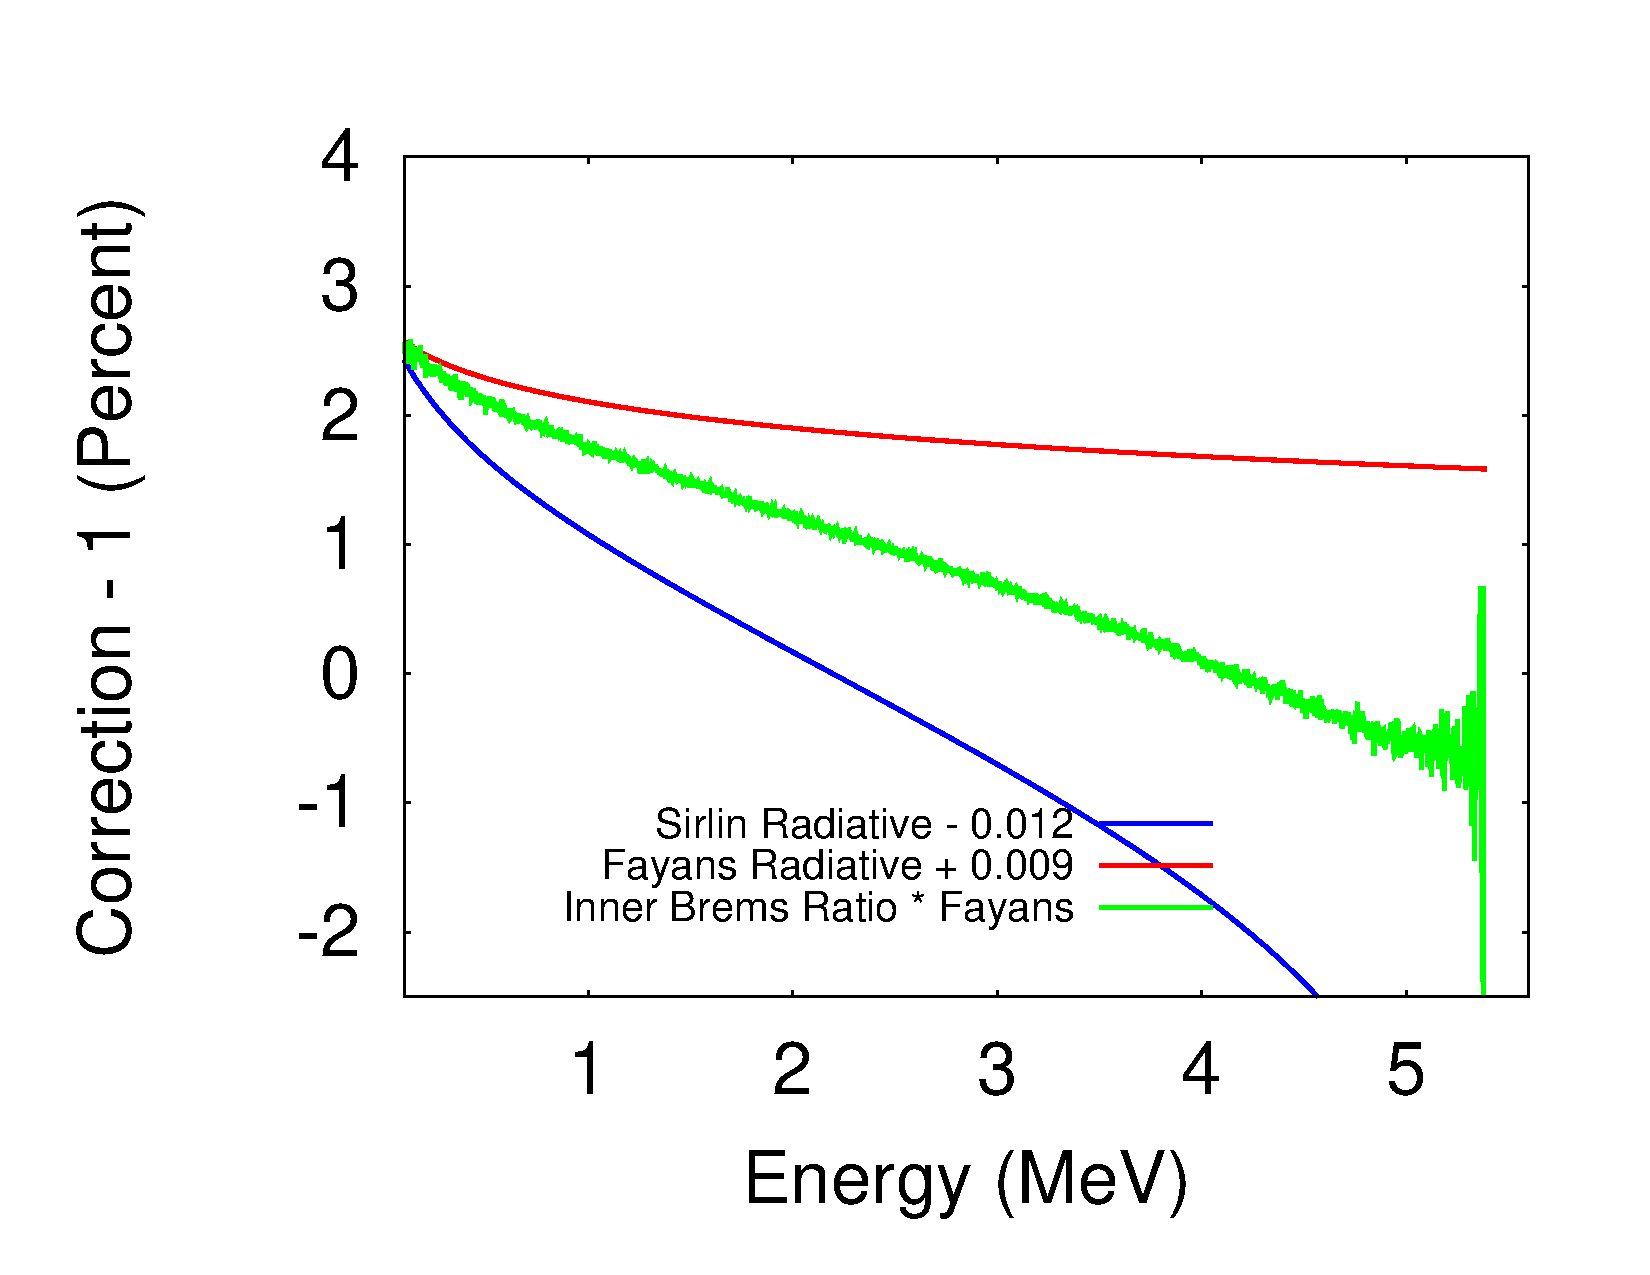
\includegraphics[width=0.78\textwidth]{RadCorrections_20F_Matching.pdf}}
	\caption{Starting all three radiative corrections from the same place.	
		 The green line is about halfway between the two others.}
	\label{fig:radmatch}
\end{figure}

\section{Screening}
The screening correction is the next largest correction.
It corresponds to the screening of the nuclear charge due to the electron cloud of the atom.
The strongest effect of the screening correction is at low electron energies.
This is a correction to the Fermi function.

\subsection{Potentials Used in Screening Derivation}
To calculate this correction, the Coulumb potential used to calculate the Fermi function is replaced with a Hulth\'en potential.
This is shown in equation \ref{eq:hulth}

\begin{equation}
	V(r) = -\frac{\alpha Z \beta}{e^{\beta r} - 1}
	\label{eq:hulth}
\end{equation}

Where $r$ is the distance away from the center and $\beta$ is a parameter characterizing the defuseness of the electron cloud.
The ratio of this new Fermi function to the old Fermi function is the screening correction.
It multiplies the phase space. 

The screening correction is negligable expect for near the origin.
Near the origin, equation \ref{eq:hulth} behaves as equation \ref{eq:hulthorg}

\begin{equation}
	V(r) = -\frac{\alpha Z}{r} + \frac{1}{2}\alpha Z \beta
	\label{eq:hulthorg}
\end{equation}

and $\beta$ is given by equation \ref{eq:screenbeta} \cite{Buh84}. 
	
\begin{equation}
	\beta = 2C(Z)\alpha Z^{\frac{1}{3}} m_{e}
	\label{eq:screenbeta}
\end{equation}

In the case of beta decay, the $Z$ is number electrons of the mother atom.
The assumption is that beta decay is occuring from neutral mother atoms.
The only unknown is $C(Z)$.

To find the value of $C(Z)$, a comparison to another method of treating screening is needed.
In another method of describing screening, the potential is described as a series of exponentials.
This is shown in \ref{eq:hart} \cite{Bya56}.

\begin{equation}
	V(r) = -\frac{\alpha Z}{r}\sum_{n}c_{n}e^{-b_{n} x}
	\label{eq:hart}
\end{equation}

where $b_{n}$ and $c_{n}$ are constants.
The sum of all the $c_{n}$ adds up to one.
The value of $x$ is shown in equation \ref{eq:screeningx} \cite{Bya56}

\begin{equation}
	x = 1.13 \alpha Z^{\frac{1}{3}} r m_{e}
	\label{eq:screeningx}
\end{equation}

When equation \ref{eq:hart} is expanded near the origin, the result is equation \ref{eq:hartorg}

\begin{equation}
	V(r) = - \frac{\alpha Z}{r} + \alpha Z 1.13 \alpha Z^{\frac{1}{3}} m_{e} \sum_{n} b_{n} c_{n}
	\label{eq:hartorg}
\end{equation}

By comparing equation \ref{eq:hulthorg}, equation \ref{eq:screenbeta} and equation \ref{eq:hartorg}, the results in equation \ref{eq:betaanswer} are obtained.

\begin{equation}
	C(Z) = 1.13 \sum_{n} c_{n} b_{n}
	\label{eq:betaanswer}
\end{equation} 

For fluorine, $n = 1$, $c = 1$, and $b = 0.907$ \cite{Bya56}.

\subsection{Screening Correction Formula}
With all these factors out of the way, the screening correction can be written.
$C(Z)$ in equation \ref{eq:screenbeta} is $0.907 * 1.13 = 1.02491$.
The result is shown in equation \ref{eq:screeningQ} \cite{Buh84}.

\begin{equation}
	Q(Z,W) = X(\frac{W'}{W})|\frac{\Gamma(\gamma + i y')}{\Gamma(\gamma+ i y)}|^{2}|\frac{\Gamma(\gamma + 2 i \frac{p'}{\beta})}{\Gamma(\gamma + 2 i \frac{p}{\beta})}|^{2}e^{-\pi y}(\frac{2p}{\beta})^{2(1 - \gamma)}

	\label{eq:screeningQ}
\end{equation}

with $y = \frac{\alpha Z W}{p}$, $y' = \frac{\alpha Z W'}{p'}$,$ \gamma$ is in table \ref{tab:vars}, $W' = W - \frac{1}{2}\alpha Z \beta$, and $p' = \frac{1}{2}p + \frac{1}{2}\sqrt{p^{2} - 2 \alpha Z W' \beta}$.

$X(\frac{W'}{W})$ is in equation \ref{eq:screeningX}

\begin{equation}
	X = \frac{1 + \frac{W' + \gamma m}{W'}\frac{\beta}{p}^{2} + \frac{1}{2}\gamma^{2}[1 + (1 - \alpha Z \beta/(W + m))^{frac{1}{2}]^{-2}[\frac{W - m}{W'}\frac{\beta}{p}^{2}[1 - \frac{1 - \gamma}{8\gamma}\frac{\beta}{p}^{2}]} {1 + \frac{\beta}{4p}^{2}}
	\label{eq:screeningX}
\end{equation}
